\documentclass[11pt]{amsart}

\usepackage[english]{babel}
\usepackage{appendix}
\usepackage{amsmath}
\usepackage{amsfonts}
\usepackage{amssymb}
%\usepackage{showlabels}
\usepackage{hyperref}
\usepackage{amsthm}
\usepackage{marginnote}
\usepackage{stmaryrd}
\usepackage{enumitem}
\usepackage[english]{babel}
\usepackage{yfonts}
\usepackage[T1]{fontenc}
\usepackage[utf8x]{inputenc}
\usepackage{verbatim}
\usepackage{graphicx}
\usepackage{verbatim}
\usepackage{faktor}
\usepackage{xcolor}
\usepackage{xfrac}
\usepackage{tikz,tikz-cd}
\usetikzlibrary{decorations.pathmorphing,decorations.pathreplacing,patterns}

\usepackage[all]{xy}
\usepackage{bbm}
\usepackage{tabularx}
\usepackage{longtable}
\usepackage{tabu}
\usepackage{booktabs}
\usepackage{mathtools}

\usepackage[]{textcomp}
\usepackage[sups]{Baskervaldx}
\usepackage{cabin}
\usepackage[varqu,varl]{inconsolata}
\usepackage[baskervaldx,bigdelims,vvarbb]{newtxmath}
\usepackage[cal=cm]{mathalfa}


\newcommand{\plC}{\scalebox{0.8}[1.3]{$\sqsubset$}}
\newcommand{\sidenote}[1]{\marginpar{\textbf{\color{red}#1}}}

\newcommand{\TT}{\operatorname{T}}
\newcommand{\oM}{\overline{\mathcal{M}}}
\newcommand{\M}[4]{\overline{\mathcal{M}}_{#1,#2}(#3,#4)}
\newcommand{\Q}[4]{\mathcal{Q}_{#1,#2}(#3,#4)}
\newcommand{\Qe}[4]{\mathcal{Q}^{\epsilon}_{#1,#2}(#3,#4)}
\newcommand{\Qt}[4]{\widetilde{\mathcal Q}_{#1,#2}(#3,#4)}
\newcommand{\QG}[4]{\mathcal{Q}G_{#1,#2}(#3,#4)}
\newcommand{\QGe}[4]{\mathcal{Q}G^{\epsilon}_{#1,#2}(#3,#4)}
\newcommand{\D}[3]{\mathcal{D^Q}(#1,#2,#3)}
\newcommand{\E}[3]{\mathcal{E^Q}(#1,#2,#3)}
\newcommand{\PP}{\mathbb P}
\newcommand{\Z}{\mathbb{Z}}
\newcommand{\tVZc}[4]{\widetilde{\mathcal{V\!Z}}^{\rm{ctr}}_{#1,#2}(#3,#4)}
\newcommand{\VZc}[4]{\mathcal{V\!Z}^{\rm{ctr}}_{#1,#2}(#3,#4)}
\newcommand{\VZcLi}[4]{\mathcal{V\!Z}^{\rm{ctr, Li}}_{#1,#2}(#3,#4)}
\newcommand{\N}{\mathbb{N}}
\newcommand{\OO}{\mathcal{O}}
\renewcommand{\to}{\rightarrow}
\newcommand{\A}{\mathcal A}
\newcommand{\B}{\mathcal B}
\newcommand{\C}{\mathfrak C}
\newcommand{\cC}{\mathcal C}
\newcommand{\EE}{\mathbf{E}}
\renewcommand{\L}{\mathcal L}
\newcommand{\LL}{\mathbf{L}}
\newcommand{\MM}{\mathfrak M}
\newcommand{\Aaff}{\mathbb{A}}
\newcommand{\kfield}{\Bbbk}
\newcommand{\comp}{\chi}
\newcommand{\sst}{\sigma^{\operatorname{ss}}}
\newcommand{\Pic}{\operatorname{Pic}}
\newcommand{\Def}{\operatorname{Def}}
\newcommand{\Spec}{\operatorname{Spec}}
\newcommand{\Proj}{\operatorname{Proj}}
\newcommand{\Hom}{\operatorname{Hom}}
\newcommand{\Ext}{\operatorname{Ext}}
\newcommand{\Gm}{\mathbb{G}_{\text{m}}}
\newcommand{\virt}[1]{[#1]^{\operatorname{virt}}}
\newcommand{\vip}[1]{[#1]^{\operatorname{prod}}}
\newcommand{\Id}{\operatorname{Id}}
\newcommand{\CC}{\mathbb{C}}
\newcommand{\QQ}{\mathbb{Q}}
\newcommand{\HH}{\operatorname{H}}
\newcommand{\Achow}{\operatorname{A}}
\newcommand{\pt}{\operatorname{pt}}
\newcommand{\bq}{\begin{equation}}
\newcommand{\eq}{\end{equation}}
\newcommand{\ba}{\begin{aligned}}
\newcommand{\ea}{\end{aligned}}
\newcommand{\be}{\begin{enumerate}}
\newcommand{\ee}{\end{enumerate}}
\newcommand{\bsm}{\left(\begin{smallmatrix}}
\newcommand{\esm}{\end{smallmatrix}\right)}                   
\newcommand{\bpm}{\begin{pmatrix}}
\newcommand{\epm}{\end{pmatrix}}
\newcommand{\barr}{\begin{displaymath}\begin{array}{cccc}}
\newcommand{\earr}{\end{array}\end{displaymath}}
\newcommand{\barrl}{\begin{displaymath}\begin{array}{lcl}}
\newcommand{\earrl}{\end{array}\end{displaymath}}
\newcommand{\barl}{\begin{displaymath}\begin{array}{l}}
\newcommand{\earl}{\end{array}\end{displaymath}}
\newcommand{\bxym}{ \begin{displaymath}\xymatrix }
\newcommand{\exym}{\end{displaymath}}
\newcommand{\bcd}{\begin{center}\begin{tikzcd}}
\newcommand{\ecd}{\end{tikzcd}\end{center}}
\newcommand{\R}{\operatorname{R}^{\bullet}}
\newcommand{\dvr}{\Delta}
%\newcommand{\sslash}{\mathbin{/\mkern-6mu/}}
\newcommand{\tr}{{\rm tr}}
\newcommand{\Isom}{\text{Isom}}
\newcommand{\pr}{\operatorname{pr}}
\newcommand{\ev}{\operatorname{ev}}
\newcommand{\codim}{\operatorname{codim}}
\newcommand{\vdim}{\operatorname{vdim}}
\newcommand{\ildef}[1]{\emph{#1}}
\newcommand{\om}[1]{\mathcal{#1}}
\newcommand{\h}{\operatorname{h}}
\newcommand{\Aut}{\operatorname{Aut}}
\newcommand{\RR}{\textbf{R}}
\newcommand{\NN}{\operatorname{N}}
\newcommand{\ovm}[1]{\overline{\mathcal{#1}}}
\newcommand{\ovt}[1]{\widetilde{\mathcal{#1}}}
\newcommand{\ov}[1]{\overline{#1}}

\theoremstyle{definition}
\newtheorem{thm}{Theorem}[section]
\newtheorem{lem}[thm]{Lemma}
\newtheorem{lemma}[thm]{Lemma}
\newtheorem{prop}[thm]{Proposition}
\newtheorem{cor}[thm]{Corollary}
\newtheorem*{teo*}{Theorem}
\newtheorem{ipotesi}{ipotesi}
\newtheorem*{nota}{Nota}
\newtheorem{claim}{Claim}
\newtheorem{question}[thm]{Question}
\newtheorem{conj}[thm]{Conjecture}

\newtheorem{innercustomthm}{Theorem}
\newenvironment{customthm}[1]
  {\renewcommand\theinnercustomthm{#1}\innercustomthm}
  {\endinnercustomthm}

\theoremstyle{definition}
\newtheorem{example}[thm]{Example}
\newtheorem{ex}[thm]{Example}
\newtheorem{dfn}[thm]{Definition}
\newtheorem{definition}[thm]{Definition}
\newtheorem{aside}[thm]{Aside}
\newtheorem{remark}[thm]{Remark}
\newtheorem{com}[thm]{Comment}
\newtheorem{num}{Number}
\newtheorem*{sketch}{Sketch}
\newtheorem*{rem}{Remark}
\newtheorem*{aside*}{Aside}
\newtheorem*{acknowledgements}{Acknowledgements}

\newcommand{\ilemph}[1]{\emph{#1}}

\setcounter{tocdepth}{1}

\newcommand{\todo}[1]{\vspace{5mm}\par \noindent
\framebox{\begin{minipage}[c]{0.95 \textwidth} \tt #1\end{minipage}} \vspace{5mm} \par}

\def\ti{-\allowhyphens}
\newcommand{\thismonth}{\ifcase\month % case 0 --- impossible!
  \or January\or February\or March\or April\or May\or June%
  \or July\or August\or September\or October\or November%
  \or December\fi}
\newcommand{\thismonthyear}{{\thismonth} {\number\year}}
\newcommand{\thisdaymonthyear}{{\number\day} {\thismonth} {\number\year}}

\title[Genus One Reduced Relative Invariants]{Relative Stable Maps in Genus One via Central Alignments}
\author{Luca Battistella, Navid Nabijou and Dhruv Ranganathan}
\date{\thismonthyear}

\begin{document}


\begin{abstract} For a smooth projective variety $X$ and a smooth very ample hypersurface $Y \subseteq X$, we define moduli spaces of relative stable maps to $(X,Y)$ in genus one, as closed substacks of the moduli space of maps from centrally aligned curves, constructed in \cite{RSPW}. We construct virtual classes for these moduli spaces, which we use to define \emph{reduced relative Gromov--Witten invariants} in genus one.

[GOALS: We prove a recursion formula which allows us to completely determine these invariants in terms of the reduced Gromov--Witten invariants, as defined in [REF]. We also prove a relative version of the Li--Zinger formula, relating our invariants to the usual relative Gromov--Witten invariants. Also say something about quasimaps.]
\end{abstract}

\maketitle

\appendixtitletocoff
\tableofcontents

\section{The space of relative centrally aligned maps}
\noindent Recall \cite{RSPW} that the moduli space of maps from centrally aligned curves is obtained by considering the  Cartesian diagram
\bcd
\tVZc{1}{n}{X}{\beta}\ar[d]\ar[r]\ar[dr,phantom,"\Box"] & \M{1}{n}{X}{\beta}\ar[d] \\
\MM_{1,n}^{\rm{ctr}}\ar[r] & \MM_{1,n}^{\dagger}
\ecd
so that objects of $\tVZc{1}{n}{X}{\beta}$ consist of
\begin{enumerate}
\item a centrally aligned curve $(C,M_C,\delta)$;
\item a stable map $f\colon C \to X$;
\end{enumerate}
subject to the condition that the subcurve $C_0 \subseteq C$, consisting of those components $C_v$ for which $\lambda(v) < \delta$, coincides with the maximal connected genus one subcurve contracted by $f$. They then define
\begin{equation*} \VZc{1}{n}{X}{\beta} \subseteq \tVZc{1}{n}{X}{\beta} \end{equation*}
to be the closed substack consisting of maps satisfying the \emph{factorisation condition}, namely that the map $f\colon C\to X$ factors through the associated contraction to a Smyth curve, i.e. there exists a map $\bar{f}$ making the following square commute:
\bcd
\widetilde C\ar[r]\ar[d] & \overline C\ar[d,"\bar f" left,dotted] \\
C\ar[r,"f"] & X
\ecd
One should think of the factorisation condition as identifying the main component of the moduli space.

\section{Definition of centrally aligned relative space}
\section{Characterisation of the closed points of the relative space}
\section{Recursion formula}

\subsection{The case $\sum\alpha=d$}

\subsection{Definition of the boundary components} According to Vakil's article there should be three sorts of boundary components.
\begin{enumerate}[label=(\alph*)]
 \item \[\mathcal Y^a=\M{0}{\lvert\alpha^{(0)}\rvert+r}{H}{d_0}\times_{H^r}\left(\VZc{1}{\alpha^{(1)}\cup\{m^{(1)}\}}{\PP^N|H}{d_1}\times\prod_{i=2}^r\M{0}{\alpha^{(i)}\cup\{m^{(i)}\}}{\PP^N|H}{d_i}\right)\]
 \item \[\mathcal Y^b=\M{0}{\lvert\alpha^{(0)}\rvert+r}{H}{d_0}\times_{H^r}\left(\M{0}{\alpha^{(1)}\cup\{m^{(1)},m^{(2)}\}}{\PP^N|H}{d_1}\times\prod_{i=3}^r\M{0}{\alpha^{(i)}\cup\{m^{(i)}\}}{\PP^N|H}{d_i}\right)\]
 \item \[\mathcal Y^c\subseteq \VZc{1}{\lvert\alpha^{(0)}\rvert+r}{H}{d_0}\times_{H^r}\prod_{i=1}^r\M{0}{\alpha^{(i)}\cup\{m^{(i)}\}}{\PP^N|H}{d_i}\]
 $\mathcal Y^c$ is cut within the latter by Gathmann's condition on line bundles:
 \[f_{|E}^*\mathcal O_H(1)\cong\mathcal O_E\left(\sum_{x_j\in E}\alpha_jx_j-\sum_{i=1}^r m^{(i)}y_i\right)\]\sidenote{Express the line bundle condition in terms of tautological classes?}
 Notice that such condition depends on the choice of $m^{(i)}$ but is really just a condition on the first factor of the product, so $\mathcal Y^c$ itself can be expressed as a product.
\end{enumerate}

\begin{remark}
 Notice that gluing does not present the subtleties to which log geometry has made us used, since we endow the curves with the minimal centrally aligned structure, possibly after prescribing that the smoothing parameters for the newly created nodes are \emph{bigger} than the contraction radius $\delta$.
\end{remark}

\begin{remark}
 A dimensional computation shows that $\mathcal Y^b$ is never relevant to the purpose of the recursion formula. On the other hand the classes of $\mathcal Y^a$ and $\mathcal Y^c$ should be weighted with the coefficient $\frac{\prod m^{(i)}}{r!}$. Let $D_{1,\alpha,k}(\PP^N|H)$ be the union of all the $\mathcal Y^a$ and $\mathcal Y^c$ as above, for any choice of number of external components $r$, distribution of the markings $A$, and of the degree $D$, provided the marked point $x_k$ lies on the internal component $C^{(0)}$. Let each component be endowed with its fundamental class weighted as above and let $\virt{D_{1,\alpha,k}(\PP^N|H)}$ be the sum of all these classes.
\end{remark}

\begin{thm}
 Assume $\sum\alpha=d$. Then \[(\alpha_k\psi_k+\ev_k^*H)[\VZc{1}{\alpha}{\PP^N|H}{d}]=\virt{D_{1,\alpha,k}(\PP^N|H)}.\]
\end{thm}
\begin{proof}
We perform a number of reductions.
 \begin{itemize}%[leftmargin=1cm]
  \item \textbf{Reduction to the case of $\PP^1|\{\infty\}$:} by choosing a general $N-2$-plane $A\subseteq H$ and projecting away from it. Must show that the rational map $\rho_A\colon \VZc{1}{n}{\PP^N|H}{d}\dashrightarrow \VZc{1}{n}{\PP^1|\{\infty\}}{d}$ is defined and smooth at a general point of $D_{1,\alpha,k}(\PP^N|H)$.
  
  \item \textbf{Reduction to an \'etale neighbourhood of $C^{(0)}$:} the plan is to understand the global perfect obstruction theory of $\VZc{1}{n}{\PP^1}{d}$ and see that the tangent to the latter is a sum of contributions from the \emph{special loci}, namely contracted components, ramification points, markings and nodes.
  
  \begin{remark}
   When we are studying the infinitesimal deformation theory of centrally aligned curves, notice that being centrally aligned must be checked on geometric points, and minimality is open, hence any deformation as a log smooth curve will automatically be minimal centrally aligned. The tangent space is then $H^1(C,T_C^{\rm{log}})$; notice that this is independent from the log structure on the base.
  \end{remark}
  
  \begin{example}
   There are non-trivial deformations that are trivial on the underlying marked prestable curve. If $(C,\mathcal M_C)\to (\Spec(k),Q^{\rm{cen}})$ is a centrally aligned curve, then in order to define a deformation over $\Spec(k[\epsilon])$ we need to extend the log structure on the base by choosing a map $Q^{\rm{cen}}\to k[\epsilon]$. Notice that if we want the underlying curve to be a trivial deformation we better send all the smoothing parameters to $0$ in $k[\epsilon]$; on the other hand, if $Q^{\rm{cen}}$ contains an element such as $e_i-e_j$ (making $R_i$ further from the circuit than $R_j$), then we are free to map it to an invertible element in $k[\epsilon]$, which will kill it in the associated log structure;\sidenote{Invertible elements of $k[\epsilon]$ remain invertible when setting $\epsilon=0$, which seems to kill $e_i-e_j$ on the central fiber too.} this will make $R_i$ and $R_j$ be \emph{at the same distance} from the circuit in the deformation. Importantly, $Q^{\rm{log}}\to Q^{\rm{cen}}$ is an epimorphism only in the category of integral monoid (of which the multiplicative monoid of a ring is never an object, because it has a sink).
  \end{example}


 \end{itemize}

\end{proof}


\appendix
\section{Old}

\subsection{Definition of the relative space} We now give a definition of the relative space inside the moduli space of centrally aligned stable maps.
\begin{dfn}
Let $X$ be a smooth projective variety with a smooth divisor $Y$. Fix a vector of tangency conditions $\alpha=(\alpha_1,\ldots,\alpha_n)$ with $\Sigma_{i=1}^n \alpha_i = Y \cdot \beta$. Then the \emph{centrally aligned relative space} 
\begin{equation*}\VZc{1}{\alpha}{X|Y}{\beta} \end{equation*}
is defined to be the closed substack of $\VZc{1}{n}{X}{\beta}$ satisfying the following conditions:
\begin{enumerate}
\item \emph{Gathmann's relative condition:} for each connected component $Z$ of $f^{-1}(Y)$, either:
\begin{enumerate}
\item $Z$ is a single point of $C$, in which case if $Z=x_i$ is a marking then we require that the multiplicity of $f$ at $x_i$ along $Y$ is at least $\alpha_i$ (if $Z$ is not a marking then there is no condition);
\item $Z$ is a subcurve $Z \subseteq C$, in which case we require that
\begin{equation*} f^*[Y]|_Z -\sum_{x_i\in Z}\alpha_ix_i\end{equation*}
is an effective class in $\Achow_0(Z)$.
\end{enumerate}

\item \emph{Compatibility condition:} this applies when the minimal subcurve of genus one (the \emph{circuit} or \emph{core}) is contracted to a point in $Y$. In this case we require that the following diagram of solid arrows may be completed to a commutative diagram:
\bcd
Q_{\rm{min}}^{\rm{prestable}}\ar[r]\ar[d] & Q_{\rm{min}}^{\rm{log.map}} \\
Q_{\rm{min}}^{\rm{cen.align}}\ar[dashed,ur]
\ecd
\end{enumerate}
\end{dfn}

\begin{remark}[Explaining Gathmann]
Gathmann's condition is promptly extended to the case that $\Sigma_{i=1}^n \alpha_i \leq Y \cdot \beta$. \textcolor{red}{Question: what is the correct generalisation of the compatibility condition?} Here we try to make the condition for a curve component of $f^{-1}(Y)$ into an easily verifiable criterion: if $Z$ is a smooth elliptic curve, recall that every line bundle of positive degree on it is effective, hence the relative condition can be rephrased as the following numerical criterion:
\begin{equation*} f_*[Z]\cdot [Y]+\sum_{j=1}^r m^{(j)}\geq \sum_{x_i\in Z}\alpha_i \end{equation*}
together with the additional requirement that, when the above is an equality, there is an isomorphism of line bundles:
\begin{equation}\label{eqn:eq_in_Pic}
(f|_{Z})^*\OO_X(Y) \otimes \OO_Z\left(\sum_{j=1}^r m^{(j)}y_j\right)=\OO_Z\left(\sum_{x_i\in Z}\alpha_ix_i\right) 
\end{equation}
 
 If $Z$ is reducible, the correct extension is not to impose the same condition componentwise; rather, we should ask the numerical condition for the total degree, and, if $Z$ is obtained by gluing a smooth elliptic curve $E$ with a forest of rational trees $T_i$ at roots $q^E_i$, then the line bundle equality \eqref{eqn:eq_in_Pic} should be required in $\Pic(E)$ after counting each $q^E_i$ towards the left hand side with multiplicity
 \[f_*[T_i]\cdot [Y]+\sum_{\text{external components attached to $T_i$}} m^{(j)}- \sum_{x_j\in T_i}\alpha_j.\]
 
 %That this is the right thing to do follows from the proof that Gathmann's relative space is the projection of Jun Li's moduli space of maps to the expanded pair after contracting the higher levels of the accordion.
\end{remark}

\begin{remark}[Explaining compatibility]
First we need to define the monoids and maps involved. We start with $Q_{\rm{min}}^{\rm{prestable}}\to Q_{\rm{min}}^{\rm{log.map}}$; when looking at a geometric point $\Spec(k=\bar k)$ it is well-known that \[ Q_{\rm{min}}^{\rm{prestable}}=\prod_{q\ \text{node}}\mathbb N_q.\]
Let us assume that all the nodes are internal, i.e. map to $Y$, for all the action happens there, and also that there is only one internal connected component $Z$, which is a curve of arithmetic genus one. Then we define $Q_{\rm{min}}^{\rm{log.map}}$ as the saturation of the quotient of
\begin{equation}\label{eq:logminmod} \prod_{q\ \text{node}}\mathbb N_q \times \prod_{S\ \text{internal irr. compo.}}\mathbb N_S\end{equation}
by the relation generated in the groupification of the latter by
\[\langle \rm{Rel}_q=(u_q,\ldots,1,\ldots,-1,\ldots),\ q\ \text{internal node} \rangle\]
where $1$ is in position $S_q^+$ (adjacent to $q$ and further from the circuit), $-1$ in position $S_q^-$ (adjacent to $q$ and closer to the circuit), and $u_q$ in position $q$ is defined as to include the tropical balancing condition (I don't know whether this is standard):
\[u_q=f_*[T_q]\cdot [Y]+\sum_{R_i \text{external compo. attached to }T_q} m^{(i)}- \sum_{x_j\in T_q}\alpha_j,\]
where $T_q$ is the tree of internal components that $q$ separates from the circuit. Notice that the nodes between $Z$ and an external component $R_i$ have no $1$, so the corresponding relations look like \[(u_q,\ldots,-1,\ldots).\]
The map $Q_{\rm{min}}^{\rm{prestable}}\to Q_{\rm{min}}^{\rm{log.map}}$ is induced by the inclusion of the node factors in \eqref{eq:logminmod}. If we call $e_q$ the image in $Q_{\rm{min}}^{\rm{log.map}}$ of the $q$-th basis vector, then we can verify that the following equations hold: chosen any internal component $S_i$ and any two external component $R_i^1, R_i^2$
such that their path to the circuit goes through $S_i$, then
\begin{equation}
 \sum_{q\in[R_i^1,S_i]}u_qe_q=\sum_{q\in[R_i^2,S_i]}u_qe_q.
\end{equation}
\textcolor{red}{Question: is this monoid factorisation condition a closed one?}
\end{remark}

\begin{remark}
 Here is a tidy example: start with an elliptic curve $E$ contracted to $Y$, with two external components $R_1, R_2$ attached to it and a single marking $x\in E$. The tropical picture would be:
\begin{center}
 \begin{tikzpicture}[radius=2pt,scale=0.5]
 \draw[fill=black] (0,0) circle;
 \draw (0,0) -- (4,0);
 \draw[fill=black] (0,2) circle;
 \draw[fill=black] (0,4) circle;
 \draw (0,2) -- (2,3);
 \draw (0,4) -- (2,3);
 \draw (2,3) -- (4,3);
 \draw[fill=white] (2,3) circle;
 \draw[->] (2,1.5) -- (2,.5);
 \end{tikzpicture}
\end{center}
The dual monoids in the compatibility condition give us the following nice picture:
\begin{center}
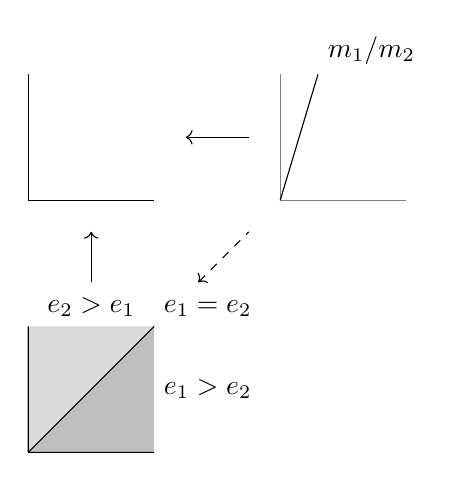
\begin{tikzpicture}[scale=0.8]
 \draw (0,0) -- (0,2)  (0,0)--(2,0);
 \draw[->] (1,-1.3) -- (1,-.5);
 \fill[gray!30] (0,-4) -- (0,-2) -- (2,-2) -- (0,-4);
 \fill[gray!50] (0,-4) -- (2,-4) -- (2,-2) -- (0,-4);
 \draw (0,-4) -- (0,-2) (0,-4) -- (2,-4) (0,-4) -- (2,-2) node[above right]{$e_1=e_2$};
 \draw (1,-2) node[above]{$e_2>e_1$} (2,-3) node[right]{$e_1>e_2$};
 \draw[<-] (2.5,1)--(3.5,1);
 \draw[gray!=30] (4,0) -- (4,2)  (4,0)--(6,0);
 \draw (4,0) -- (4.6,2) node[above right]{$m_1/m_2$};
 \draw[<-,dashed] (2.7,-1.3)--(3.5,-.5);
\end{tikzpicture}
\end{center}
So, for example, the factorisation exists for the subcone $e_2>e_1$ only when $m_1>m_2$, which is compatible with the fact that $\mathbb N^2=Q_{\rm{min}}^{\rm{prestable}}\to Q_{\rm{min}}^{\rm{log.map}}=\mathbb N$ is given by
$e_1\mapsto m_2, e_2\mapsto m_1$.
\end{remark}


\section{The relative space is the closure of the nice locus for $(\PP^N,H)$}
\noindent In general we do not know very much about the space we have just defined. The aim of this section is to show that, in the case where $X=\PP^N$ and $Y=H$ is a hyperplane, the space is proper and irreducible of the expected dimension. As such it has a fundamental class, which we can use to define reduced relative Gromov--Witten invariants in genus one.

\begin{remark} In the case of a general pair $(X,Y)$ we will see that the moduli space is still proper, but is not in general irreducible or even equidimensional. Nevertheless, we can equip it with a virtual class by ``pulling back'' from the case of $(\PP^N,H)$; for details, see \S [REF]. \end{remark}

The strategy is as follows. We define (Definition \ref{Definition of nice locus}) an open subspace
\begin{equation*}\VZc{1}{\alpha}{\PP^N|H}{d}^{\circ} \subseteq \VZc{1}{\alpha}{\PP^N|H}{d}\end{equation*}
called the \emph{nice locus}, on which the source curve and the map take a particularly simple form. Because of this simplicity, it is easy to show that the nice locus is irreducible (Lemma \ref{Nice locus is irreducible}). We then prove that $\VZc{1}{\alpha}{\PP^N|H}{d}$ is equal to the closure of the nice locus inside $\VZc{1}{n}{\PP^N}{d}$. Thus it is proper, since it is a closed subspace of a proper space, and it is irreducible, since it is the closure of an irreducible space.

\begin{definition} \label{Definition of nice locus} The \emph{nice locus} is defined as the open substack
\begin{equation*}\VZc{1}{\alpha}{\PP^N|H}{d}^{\circ} \subseteq \VZc{1}{\alpha}{\PP^N|H}{d}\end{equation*}
of centrally aligned maps satisfying the following two conditions:
\begin{enumerate}
\item the source curve $C$ is irreducible;
\item $f$ does not map $C$ inside $H$.
\end{enumerate}
\end{definition}

\begin{lem}\label{Nice locus is irreducible}
The nice locus $\VZc{1}{\alpha}{\PP^N|H}{d}^{\circ}$ is irreducible.
\end{lem}
\begin{proof}
By definition the contraction radius $\delta$ is compatible with the map, i.e. the subcurve $C_0\subseteq C$ where $\lambda<\delta$ is equal to the maximal connected genus one subcurve contracted by $f$. Hence when the source curve is irreducible we must have $\delta=0$, and we see that the central alignment on $C$ is uniquely and trivially determined. Thus to specify a point in the nice locus we only need to specify the source curve $C$ (as a scheme) and the map $f$. A parametrisation can be given from the vector bundle:
\[ \operatorname{Vb}\left(\pi_*\OO_{\mathcal E}(\sum_{j=n+1}^{n+\delta}\sigma_j)\oplus\pi_*\OO_{\mathcal E}(\sum_{j=1}^{n+\delta}\sigma_j)^{\oplus r}\right) \quad \text{on} \quad \mathcal{M}_{1,n+\delta}\]
where $\pi\colon\mathcal E\to\mathcal M$ is the universal curve and $\delta=d-\sum\alpha_i$.
\end{proof}

\subsection{Justifying the novel condition by dimensional reasons}
Here is a dimensional computation in an explicit example which shows that being in the closure of the nice locus must impose some condition on the log structure.
\begin{example}
Consider $\M{1}{(3)}{\PP^1|H}{3}$. This moduli space has virtual dimension $6+1-3=4$. Here is a parametrisation of the nice locus: choose an object $(E,p) \in \mathcal{M}_{1,1}$, and let $s_0$ be the natural section $s_0 \colon\OO_E\hookrightarrow\OO_E(3p)$ and $s_1$ any other section of $\OO_E(3p)$ not vanishing at $p$ (notice that $\h^0(E,\OO_E(3p))=3$). Then $(E,p,[\lambda s_0,s_1])$ gives a well-defined element of the nice locus for $\lambda \neq 0$.

Consider now the following weighted graph for a map in the boundary
\begin{center}
\begin{tikzpicture}
\draw[color=brown] (0,0) node[left]{$E$} -- (4,0);
\draw[fill=black] (1,0) circle[radius=2pt] node[above]{$x_1$};
\draw[fill=black] (2,0) circle[radius=2pt] node[below right]{$y_1$};
\draw[fill=black] (3,0) circle[radius=2pt] node[below right]{$y_2$};
\draw (2,1.5) node[left]{$R_1$} (3,1.5) node[left]{$R_2$};
\draw (2,-1) -- (2,2) node[above]{$2$} (3,-1) -- (3,2) node[above]{$1$};
\draw[->] (5,0.5) -- (8,0.5);
\draw (9,-1) -- (9,2) node[above]{$\PP^1$};
\draw[fill=black] (9,0) circle[radius=2pt] node[right]{$H$};
\end{tikzpicture}
\end{center}
where the brown line represents a contracted genus $1$ curve. Now $(E,x_1,y_1,y_2)$ is a point of $\mathcal{M}_{1,3}$ subject to the divisorial condition $3x_1-2y_1-y_2=0\in \Achow_0(E)$; furthermore we have to choose the second branch point of the $2:1$ map from $R_1$ to $\PP^1$. This already makes up for a $3$-dimensional moduli space of degenerate relative maps corresponding to such a graph. The minimal log structure for this curve has a chart from $\mathbb N^2$, with generators $e_1$ and $e_2$ corresponding to the smoothing parameters of the two nodes. If we allowed $e_1$ and $e_2$ to be identified in the characteristic sheaf, then we would get an extra $\Gm$ of choices for the log structure, so in total a $4$-dimensional moduli space. Thus if we don't impose the novel condition then we get a whole other component of the relative space, which of course for dimensional reasons cannot be contained in the closure of the nice locus.\qed
\end{example}

\begin{remark}
 For the reader who is unfamiliar with centrally aligned log curves, it might be convenient to recall that they provide a modular interpretation of the iterated blow-up procedure of Vakil and Zinger. In particular it is natural that not all of the exceptional divisors be contained in the closure of the nice locus for every $\alpha$; this geometric information is contained in the compatibility condition.
\end{remark}

\subsection{Proof sketch} \textcolor{red}{The compatibility condition should imply that the map admits a log-enhancement;} if we can prove that there is a smooth, connected and proper moduli space above, then we automatically get that the Gathmann-like relative space is closed and irreducible, and it obviously contains the nice locus; hence, if we can prove that the latter is dense, we win.

It thus remains to show that, given a relative centrally aligned map, we can smooth it to one in the nice locus. The only interesting case \textcolor{red}{should be} that the core is contracted to a point of $Y$. Here is how we prove it:
\begin{enumerate}
 \item we consider the core (say it's a smooth elliptic curve) marked with all the special points (markings and nodes); consider $E\times\dvr$ and blow it up in all the points of the central fiber that originally corresponded to nodes; we carefully and iteratively blow up smooth points of the central fiber in order to reconstruct the curve $C$ that we started with. In fact we may perform weighted instead of ordinary blow-ups, picking the ideal $(z,t^r)$ where $z$ is a vertical coordinate; this has the effect of introducing an $A_{r-1}$ surface singularity at the corresponding node of the central fiber. We do so by choosing a homomorphism $Q_{\rm{min}}^{\rm{log.map}}\to\mathbb N$ and composing it with $Q_{\rm{min}}^{\rm{prestable}}\to Q_{\rm{min}}^{\rm{log.map}}$ to determine the relevant $r$ for every node.
 \item Let $E,S_1,\ldots,S_k$ be the irreducible components of $f^{-1}(Y)$; we define a line bundle on the smoothing by
 \[\mathcal L=\OO_{\cC}\left(\sum \gamma_iS_i\right)\left(\sum \alpha_ix_i\right).\]
 Using intersection theory on the surface (recall that the local multiplicity of intersection of the two branches of the node underlying an $A_{r-1}$ singularity is $\frac{1}{r}$) we check that the compatibility condition is precisely what we need in order to be able to choose $\gamma_i$ adequately so that the following equations hold:
 \begin{align*}
  0&=\deg(\mathcal L_{|S_i}) \\
  m^{(i)}&=\deg(\mathcal L_{|R_i}) \\
  \mathcal O_E&\cong\mathcal L_{|E}
 \end{align*}
 the last from Gathmann's condition.
 \item It is not clear that sections of $\mathcal L$ are unobstructed. In order to extend them we pass to $\overline{\mathcal C}$.
\end{enumerate}

\subsection{Basic facts about centrally aligned curves}
\begin{prop}[{\cite[Proposition 4.6.2.2]{RSPW}}]
The morphism $\MM^{\rm{ctr}}_{1,n}\to\MM^{\dagger}_{1,n}$ is a log-modification.
\end{prop}

Explanation: this is a local statement so I can probably reduce to an atomic neighbourhood $S$ of a point $p$. $S$ and the curve over it are endowed with the minimal log structure; let $P=\oM_p$ determine a chart for this log structure. Observe that the subcurve $\plC_0$ of the tropicalisation $\plC$ of $C_p$ determines a subset $\rm{MinPos}$ of the set of vertices, namely those adjacent to $\plC_0$. Perform the following log-blowups: consider the set of primitive values of the function $\lambda\colon \plC\to P$, and blow up the ideal that they generate; now locally the set of values of $\lambda$ is principal with generator $p$: blow up the ideal generated by $\{\lambda(v)-p\}\setminus\{-p\}$. Keep going until $\lambda(v_i)$ is reached for some $v_i\in\rm{MinPos}$; at this point stop and declare the contraction radius $\delta:=\lambda(v_i)$. Finish by adjoining $\lambda(v)-\delta$ for all the vertices untouched to this stage. This shows that the choice of $\delta$ is not an extra degree of freedom.\marginpar{do I sound like a physicist?}

\subsection{Moral justification of the novel condition}

\begin{example} In this example we will give further moral justification for the novel condition, using as motivation the expanded degenerations approach to relative stable maps. This is not strictly necessary for what we want to do (since our spaces don't involve expanded degenerations), but it helps to explain where this condition comes from.

So, let us pretend that we have a good definition of the ``centrally aligned Li space'' of maps from centrally aligned curves to expanded degenerations:
\begin{equation*} \VZcLi{1}{\alpha}{X|D}{\beta} \end{equation*}
Objects of this moduli space should consist of maps $C \to X_l$ where $X_l \to X$ is an expansion (of some length $l$) of the pair $(X,D)$, together with a central alignment on $C$ which is compatible with this map. The factorisation property should say that the following diagram commutes:
\bcd
& \tilde{C} \ar[ld,"\nu" left] \ar[rd,"\tau"] & \\
C \ar[d,"f" left] & & \overline{C} \ar[d,"\overline{f}", dotted] \\
X_l \ar[rd,"\pi"] & & X_l \ar[ld,"\pi"] \\
& X & 
\ecd
Morally speaking, the projection map
\begin{equation*} \pi_* \colon \VZcLi{1}{\alpha}{X|D}{\beta} \to \VZc{1}{n}{X}{\beta} \end{equation*}
should have as its image our space $\VZc{1}{\alpha}{X|D}{\beta}$. We will see that everything in the image of this space must satisfy the novel condition, thus providing further justification for us imposing it.

We proceed by contradiction. Consider a genus one map $C \to \PP^1$ of the following form
\begin{center}
\begin{tikzpicture}
\draw[fill=black] (0,0) node[left]{$E$} -- (4,0);
\draw[fill=black] (0.7,0) circle[radius=2pt] node[below]{$5$};
\draw[fill=black] (2,0) circle[radius=2pt] node[above right]{$2$};
\draw[fill=black] (3,0) circle[radius=2pt] node[above right]{$3$};
\draw (2,1.5) node[right]{$C_1$};
\draw (3,1.5) node[right]{$C_2$};
\draw (2,-1) -- (2,2) node[above]{$2$};
\draw (3,-1) -- (3,2) node[above]{$3$};

\draw[->] (4.5,0) -- (6.5,0);
\draw (5.5,0) node[above]{$f$};
\draw (7,-1) -- (7,2) node[above]{$\PP^1$};
\draw[fill=black] (7,0) circle[radius=2pt] node[right]{$\infty$};
\end{tikzpicture}
\end{center}
and equip the source curve $C$ with a central alignment which identifies the lengths of the components $C_1$ and $C_2$:
\begin{center}
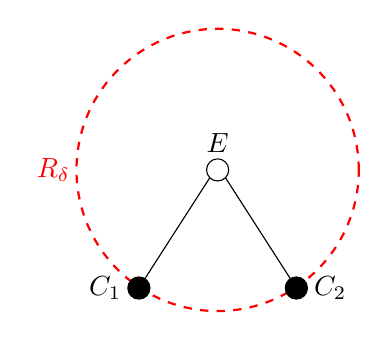
\begin{tikzpicture}
\draw[red,thick,dashed] (0,0) circle[radius=51pt];
\draw[red] (-1.75,0) node[left]{$R_\delta$};
\draw[fill=white] (0,0) circle[radius=4pt];
\draw (0,0.1) node[above]{$E$};
\draw[fill=black] (-1,-1.5) circle[radius=4pt];
\draw (-1.1,-1.5) node[left]{$C_1$};
\draw[fill=black] (-0.1,-0.1) -- (-1,-1.5);
\draw[fill=black] (1,-1.5) circle[radius=4pt];
\draw (1.1,-1.5) node[right]{$C_2$};
\draw[fill=black] (0.1,-0.1) -- (1,-1.5);
\end{tikzpicture}
\end{center}
This defines an ``object'' of $\VZc{1}{(5)}{\PP^1|\infty}{5}$, satisfying all the necessary conditions \emph{except for the novel condition}. We will show that this cannot belong to the image of $\pi_*$.

First we have to identify what the possible lifts of this object to the centrally aligned Li space are. The map $C \to X_1$ takes the following form:

\begin{center}
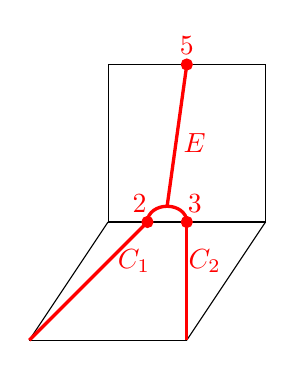
\begin{tikzpicture}
\draw (-1,-1) -- (1,-1);
\draw (-1,-1) -- (-1,1);
\draw (1,-1) -- (1,1);
\draw (-1,1) -- (1,1);
\draw (-1,-1) -- (-2,-2.5);
\draw (-2,-2.5) -- (0,-2.5);
\draw (0,-2.5) -- (1,-1);
\draw[red,very thick] (-2,-2.5) -- (-0.5,-1);
\draw[red] (-1,-1.5) node[right]{$C_1$};
\draw[red,fill=red] (-0.5,-1) circle[radius=2pt];
\draw[red] (-0.6,-1) node[above]{$2$};

\draw[red,very thick] (0,-2.5) -- (0,-1);
\draw[red] (-0.1,-1.5) node[right]{$C_2$};
\draw[red,fill=red] (0,-1) circle[radius=2pt];
\draw[red] (0.1,-1) node[above]{$3$};

\draw[red,very thick] (-0.5,-1) to [out=90,in=180] (-0.25,-0.8) to [out=0,in=90] (0,-1);
\draw[red,very thick] (-0.25,-0.8) -- (0,1);
\draw[red] (0.1,0) node{$E$};
\draw[red,fill=red] (0,1) circle[radius=2pt] node[above]{$5$};
\end{tikzpicture}
\end{center}
(Here we use Navid's convention for drawing maps to expanded degenerations, so that the box at level $1$ represents a \emph{single fibre} of the expanded degeneration, i.e. $E$ is mapped into a fibre and has zero horizontal degree.) Now, $\widetilde{C}$ is obtained from $C$ by bubbling a rational component $C_3$ at the single marking, and so the map $\widetilde{C} \to X_2$ is given by:
\begin{center}
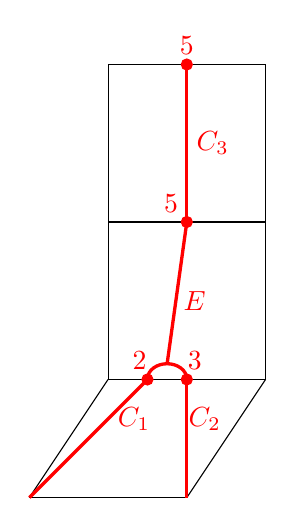
\begin{tikzpicture}
\draw (-1,-1) -- (1,-1);
\draw (-1,-1) -- (-1,1);
\draw (1,-1) -- (1,1);
\draw (-1,1) -- (1,1);
\draw (-1,-1) -- (-2,-2.5);
\draw (-2,-2.5) -- (0,-2.5);
\draw (0,-2.5) -- (1,-1);
\draw (-1,1) -- (-1,3);
\draw (-1,3) -- (1,3);
\draw (1,3) -- (1,1);
\draw[red,very thick] (-2,-2.5) -- (-0.5,-1);
\draw[red] (-1,-1.5) node[right]{$C_1$};
\draw[red,fill=red] (-0.5,-1) circle[radius=2pt];
\draw[red] (-0.6,-1) node[above]{$2$};

\draw[red,very thick] (0,-2.5) -- (0,-1);
\draw[red] (-0.1,-1.5) node[right]{$C_2$};
\draw[red,fill=red] (0,-1) circle[radius=2pt];
\draw[red] (0.1,-1) node[above]{$3$};

\draw[red,very thick] (-0.5,-1) to [out=90,in=180] (-0.25,-0.8) to [out=0,in=90] (0,-1);
\draw[red,very thick] (-0.25,-0.8) -- (0,1);
\draw[red] (0.1,0) node{$E$};
\draw[red,fill=red] (0,1) circle[radius=2pt];
\draw[red] (-0.2,1) node[above]{$5$};

\draw[red, very thick] (0,1) -- (0,3);
\draw[red] (0,2) node[right]{$C_3$};
\draw[red,fill=red] (0,3) circle[radius=2pt] node[above]{$5$};
\end{tikzpicture}
\end{center}
The map $\widetilde{C} \to \overline{C}$ contracts the elliptic component $E$, and so the map $\overline{C} \to X_1$ \emph{should} take the form:
\begin{center}
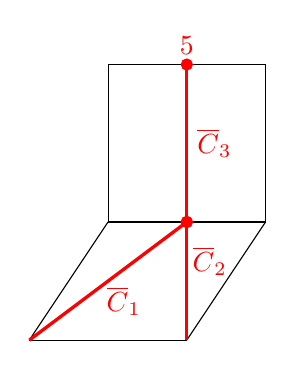
\begin{tikzpicture}
\draw (-1,-1) -- (1,-1);
\draw (-1,-1) -- (-1,1);
\draw (1,-1) -- (1,1);
\draw (-1,1) -- (1,1);
\draw (-1,-1) -- (-2,-2.5);
\draw (-2,-2.5) -- (0,-2.5);
\draw (0,-2.5) -- (1,-1);
\draw[red,very thick] (-2,-2.5) -- (0,-1);
\draw[red] (-0.8,-1.7) node[below]{$\overline{C}_1$};
\draw[red,fill=red] (0,-1) circle[radius=2pt];

\draw[red,very thick] (0,-2.5) -- (0,-1);
\draw[red] (-0.05,-1.5) node[right]{$\overline{C}_2$};
\draw[red,fill=red] (0,-1) circle[radius=2pt];

\draw[red,very thick] (0,-1) -- (0,1);
\draw[red] (0.35,0) node{$\overline{C}_3$};
\draw[red,fill=red] (0,1) circle[radius=2pt] node[above]{$5$};
\end{tikzpicture}
\end{center}
We will now see that, in this example, the map drawn above cannot actually exist, and that this occurs precisely because we have violated the novel condition.

We start by choosing a one-parameter smoothing $\mathcal{C} \to \Aaff^1$ of the centrally aligned curve $C$. This induces one-parameter smoothings $\widetilde{\mathcal{C}}$ of $\widetilde{C}$ and $\overline{\mathcal{C}}$ of $\overline{C}$. Since the factorisation condition must also hold in families, we must have a map $\overline{\mathcal{C}} \to \mathfrak{X}$, whose general fibre maps to the space $X_0=X$ (with no expansion) and whose general fibre maps to $X_1=X \sqcup_D Y$.

We thus have a map $\ovm{C} \to \mathfrak{X}$, where $\mathfrak{X}$ is the total space of the expanded degeneration. This is obtained as the toric blow-up of $\PP^1 \times \Aaff^1$ at the point $(\infty,0)$. Thus it is also a smooth toric variety, with fan given by:
\begin{center}
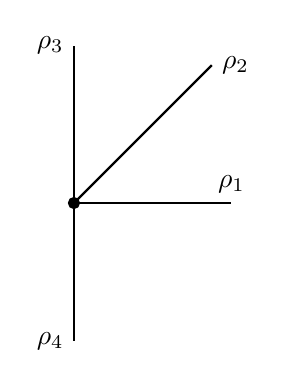
\begin{tikzpicture}
\draw[fill=black] (0,0) circle[radius=2pt];
\draw[thick] (0,0) -- (2,0) node[above]{$\rho_1$};
\draw[thick] (0,0) -- (1.75,1.75) node[right]{$\rho_2$};
\draw[thick] (0,0) -- (0,2) node[left]{$\rho_3$};
\draw[thick] (0,0) -- (0,-1.75) node[left]{$\rho_4$};
\end{tikzpicture}
\end{center}
There is a map $\mathfrak{X} \to \Aaff^1$ whose general fibre is isomorphic to $X$ and whose central fibre is isomorphic to $X_1$. We see from the fan above that $\Pic(\mathfrak{X})$ is generated by $\OO_{\mathfrak{X}}(D_{\rho_i})$ for $i=1,\ldots,4$, subject to the relations:
\begin{align*}
\OO_{\mathfrak{X}}(D_{\rho_1}) \otimes \OO_{\mathfrak{X}}(D_{\rho_2}) & \cong \OO_{\mathfrak{X}} \\
\OO_{\mathfrak{X}}(D_{\rho_2}) \otimes \OO_{\mathfrak{X}}(D_{\rho_3}) & \cong \OO_{\mathfrak{X}}(D_{\rho_4})
\end{align*}
Choosing as $\{\OO_{\mathfrak{X}}(D_{\rho_1}), \OO_{\mathfrak{X}}(D_{\rho_3})\}$ our minimal set of generators, we see that a map $\overline{\mathcal{C}} \to \mathfrak{X}$ is given by the data of line bundes $L_1$ and $L_3$ on $\overline{\mathcal{C}}$ together with sections:
\begin{align*}
s_1 & \in \HH^0(\overline{\mathcal{C}},L_1) \\
s_2 & \in \HH^0(\overline{\mathcal{C}},L_1^{-1}) \\
s_3 & \in \HH^0(\overline{\mathcal{C}},L_3) \\
s_4 & \in \HH^0(\overline{\mathcal{C}},L_1^{-1}\otimes L_3)
\end{align*}
The divisors $D_{\rho_1}$ and $D_{\rho_2}$ are, respectively, the level-$0$ and level-$1$ pieces of the central fibre of $\mathfrak{X}$. Therefore we must have
\begin{align*} & L_1 \cong \OO_{\overline{\mathcal{C}}}(a_1 \ov{C}_1 + a_2 \ov{C}_2) \\
& L_1^{-1} \cong \OO_{\ov{C}}(a_3 \ov{C}_3)
\end{align*}
for some positive integers $a_1,a_2$ and $a_3$. Here we are using the fact that each $\ov{C}_i$ is a $\QQ$-Cartier divisor on $\ovm{C}$, so that (after possibly multipltying by some positive integer) the corresponding line bundle makes sense. Furthermore, the intersection multiplicites of $\ov{C}_1$ and $\ov{C}_2$ with the level-$1$ piece mean that we must have:
\begin{align*} \deg(L_1^{-1}|_{\ov{C}_1}) & = 2\\
\deg(L_1^{-1}|_{\ov{C}_2}) & = 3 \end{align*}
We thus obtain:
\begin{align*} a_3 (\ov{C}_1 \cdot \ov{C}_3)&  = 2 \\
a_3 (\ov{C}_2 \cdot \ov{C}_3)& = 3 \end{align*}
However, we claim that in fact $\ov{C}_1 \cdot \ov{C}_3 = \ov{C}_2 \cdot \ov{C}_3$, so that the above equations cannot hold. To calculate these intersection numbers, we pass to the semistable model of $\ovm{C}$. This is obtained by performing further blow-ups to $\ovt{C}$, resulting in a semistable model $\ovt{C}^{\operatorname{ss}}$of the following form:
\begin{center}
\begin{tikzpicture}
\draw (-3,-3) -- (-3,2);
\draw (-3,-2.5) node[left]{$E$};

\draw (-3.5,1.5) -- (-0.5,1.5);
\draw (-1.3,1.725) -- (0.5,0.5);
\draw[fill=black] (0.8,0.5) circle[radius=0.5pt];
\draw[fill=black] (0.9,0.5) circle[radius=0.5pt];
\draw[fill=black] (1,0.5) circle[radius=0.5pt];
\draw (3,1.725) -- (1.2,0.5);
\draw (1.9,0.9) node[right]{$R_1^1$};
\draw (2.5,1.5) -- (5,1.5);
\draw (4,1.5) node[below]{$R_1$};

\draw (-3.5,0) -- (-0.5,0);
\draw (-1.3,0.225) -- (0.5,-1);
\draw[fill=black] (0.8,-1) circle[radius=0.5pt];
\draw[fill=black] (0.9,-1) circle[radius=0.5pt];
\draw[fill=black] (1,-1) circle[radius=0.5pt];
\draw (3,0.225) -- (1.2,-1);
\draw (1.9,-0.6) node[right]{$R_2^1$};
\draw (2.5,0) -- (5,0);
\draw (4,0) node[below]{$R_2$};

\draw (-3.5,-1.5) -- (-0.5,-1.5);
\draw (-1.3,-1.275) -- (0.5,-2.5);
\draw[fill=black] (0.8,-2.5) circle[radius=0.5pt];
\draw[fill=black] (0.9,-2.5) circle[radius=0.5pt];
\draw[fill=black] (1,-2.5) circle[radius=0.5pt];
\draw (3,-1.275) -- (1.2,-2.5);
\draw (2.5,-1.5) -- (5,-1.5);
\draw (4,-1.5) node[below]{$R_3$};
\end{tikzpicture}
\end{center}
Here the component labeled $E$ is smooth elliptic and all the other components are smooth rational. The projection $\pi: \ovt{C}^{\operatorname{ss}} \to \ovm{C}$ sends each $R_i$ to $\ov{C}_i$ and contracts all the other components. The semistable model has the advantage that the total space is regular, so the intersections are precisely those that you ``see'' in the picture. In particular, any two adjacent components have intersection $1$, and the self-intersection of any component is equal to minus the number of adjacent components.

Now, $\ov{C}_i \cdot \ov{C}_j = (\pi^* \ov{C}_i)\cdot(\pi^* \ov{C}_j)$, so we want to show that:
\begin{equation*} (\pi^* \ov{C}_1)\cdot(\pi^*\ov{C}_3) = (\pi^* \ov{C}_2)\cdot(\pi^*\ov{C}_3) \end{equation*}
For each $i$, $\pi^*\ov{C}_i$ is equal to $R_i$ plus a non-negative linear combination of the components in $\ovt{C}^{\operatorname{ss}}$ contracted by $\pi$. By the projection formula, any component contracted by $\pi$ will multiply to zero with a class pulled back along $\pi$. Thus
\begin{equation*} (\pi^* \ov{C}_1)\cdot(\pi^*\ov{C}_3) = R_1 \cdot (\pi^*\ov{C}_3) = a_3(R_1^1) \end{equation*}
the coefficient of $R_1^1$ in $\pi^* \ov{C}_3$. Similarly
\begin{equation*} (\pi^* \ov{C}_2) \cdot (\pi^* \ov{C}_3) = a_3(R_2^1) \end{equation*}
the coefficient of $R_2^1$ in $\pi^* \ov{C}_3$. So we need to show that:
\begin{equation*} a_3(R_1^1) = a_3(R_1^2) \end{equation*}
Now, we have
\begin{equation*} 0 = R_1^1 \cdot (\pi^* \ov{C}_3) = a_3(R_1^2) - 2a_3(R_1^1) \end{equation*}
because $(R_1^1)^2=-2$. So $a_3(R_1^1) = a_3(R_1^2)/2$. Similarly:
\begin{equation*} 0 = R_1^2 \cdot (\pi^*\ov{C}_3) = a_3(R_1^1) - 2a_3(R_1^2) + a_3(R_1^3) = -3a_3(R_1^1) + a_3(R_1^3) \end{equation*}
So $a_3(R_1^1) = a_3(R_1^3)/3$. Continuing in this way, we find that
\begin{equation*} a_3(R_1^1) = a_3(E)/l_1 \end{equation*}
where $l_1$ is the length of the rational tail connecting $E$ to $R_1$. Similarly $a_3(R_1^2) = a_3(E)/l_2$. But by Smyth's balancing condition for the semistable model \cite[Proposition 2.11]{SMY1}, we must have $l_1=l_2$. This concludes the proof that $\ov{C}_1 \cdot \ov{C}_3 = \ov{C}_2 \cdot \ov{C}_3$, which shows the necessity of the novel condition in this example.

Notice that here we used the fact that the rational tails $\ov{C}_1$ and $\ov{C}_2$ are adjacent to the same irreducible component (namely $E$) of the core.\qed
\end{example}

\subsection{Proof that the relative space equals the closure of the nice locus.}
We now want to show that the relative space in the centrally aligned setting is equal to the closure of the nice locus; irreducibility then follows immediately. We start with one direction:

\begin{lem}
The closure of the nice locus is contained in the relative space.
\end{lem}
\begin{proof}
We address the relative conditions one at a time. Notice that they are all obviously satisfied on the nice locus. Also, Gathmann's relative condition is obviously closed; see \cite[Proposition 4.9]{Vre}.

It remains to show that the novel condition is satisfied on the closure of the nice locus. Here is no proof but rather some heuristics. Consider for example a map similar to the one above
\begin{center}
\begin{tikzpicture}
\draw[color=brown] (0,0) node[left]{$E$} -- (4,0);
\draw[fill=black] (1,0) circle[radius=2pt] node[above]{$x_1$};
\draw[fill=black] (2,0) circle[radius=2pt] node[below right]{$y_1$};
\draw[fill=black] (3,0) circle[radius=2pt] node[below right]{$y_2$};
\draw (2,1.5) node[left]{$R_1$} (3,1.5) node[left]{$R_2$};
\draw (2,-1) -- (2,2) node[above]{$3$} (3,-1) -- (3,2) node[above]{$2$};
\draw[->] (5,0.5) -- (8,0.5);
\draw (9,-1) -- (9,2) node[above]{$\PP^1$};
\draw[fill=black] (9,0) circle[radius=2pt] node[right]{$H$};
\draw[fill=black] (9,1.5) circle[radius=2pt] node[right]{$H'$};
\end{tikzpicture}
\end{center}
and assume that it is in the closure of the nice locus; I want to argue that the two smoothing parameters cannot be identified. By the previous points I may assume that the factorisation property and Gathmann's relative conditions hold. I have a diagram:
\bcd
\cC^{\rm{ss}}\ar[r]\ar[dr] & \widetilde \cC\ar[r]\ar[d] & \overline \cC\ar[d,"\bar f"] \\
& \cC\ar[r,"f"] & X
\ecd
where I have included the semistable model of $\cC$ (and $\widetilde \cC$), thought of as a curve marked with $f^{-1}(H')$ as well, where $H\neq H'\in\PP^1$.

Notice that $\cC$ is a normal surface with at worst singular points at the nodes of $C=\cC_0$ (the central fibre $C=E+R_1+R_2$ is Cartier and a variety is smooth at any smooth point of a Cartier divisor) and the singularities are of type $A_{n_i},\ i=1,2$ (from the deformation theory of nodal curves).

I assume maximal multiplicity $\sum\alpha=d$, i.e. I am looking at the moduli space $\M{1}{(5)}{\PP^1|H}{5}$. Hence the line bundle and $s_0$ are determined as $f^*\OO_{\PP^1}(1)=\OO_{\cC}(5x_1)\otimes\OO_{\cC}(\beta E)$ for some (positive rational) $\beta$ and $s_0$ is the natural inclusion of $\OO_{\cC}$ (up to $\Gm$). 

The map is totally ramified at $y_i$ by Gathmann's condition. We conclude:
\[ \frac{\beta}{n_i+1}=(\beta E)\cdot R_i=m^{(i)}\]
Hence, having fixed the multiplicities, the two possible singularities of $\cC$ determine each other. In our example we may pick $n_1=1,\ n_2=2,\ \beta=6$. But knowing the singularity determines the semistable model: in our case $y_1$ is replaced by a $(-2)$-curve and $y_2$ by a chain of two $(-2)$-curves. Now we know from the work of Smyth \cite[Proposition 2.12]{SMY1} that the exceptional locus of $\cC^{\rm{ss}}\to\overline\cC$ is balanced, therefore we may deduce that $\bar f$ is constant on the branch of the genus $1$ singularity to which $R_2$ is joined, so $\overline C$ looks like this:

\begin{center}
\begin{tikzpicture}
\draw (-1,0) -- (1,0) node[right]{$\overline R_1$};
\draw[color=gray!50] (-1,-1) -- (1,1);
\draw[fill=black] (-.75,-.75) circle[radius=2pt] node[left]{$x_1$};
\draw[color=gray!50] (0,-1) -- (0,1);
\draw (-1,1.5) node[above left]{$\overline R_2$} -- (.25,.5);
\end{tikzpicture}
\end{center}
where a gray line is contracted by the map. On the other hand if $\delta=\lambda(v_1)=\lambda(v_2)$ then the prescription of \cite[Proposition 3.6.1]{RSPW} implies that $\tilde C\to \overline C$ looks like:
\begin{center}
\begin{tikzpicture}
\draw[color=brown] (0,0) node[left]{$E$} -- (4,0);
\draw[color=gray!50] (1,-1) -- (1,2);
\draw[fill=black] (1,1) circle[radius=2pt] node[left]{$x_1$};
\draw (2,1.5) node[left]{$R_1$} (3,1.5) node[left]{$R_2$};
\draw (2,-1) -- (2,2) node[above]{$3$} (3,-1) -- (3,2) node[above]{$2$};
\draw[->] (5,0.5) -- (7,0.5);
\draw (8,0.5) -- (10,0.5) node[right]{$\overline R_1$};
\draw[color=gray!50] (8,-.5) -- (10,1.5);
\draw[fill=black] (8.25,-.25) circle[radius=2pt] node[left]{$x_1$};
\draw (9,-.5) -- (9,1.5) node[above left]{$\overline R_2$};
\end{tikzpicture}
\end{center}
which is a contradiction.
\end{proof}

\subsection{Novel Condition 2.0}

This is done with $(\PP^1,H)$ in mind; in general it will need to be modified to account for internal components of positive degree.

\textbf{Novel condition 2.0:} if $v_1,v_2$ are two vertices belonging to $R_\delta$, then the corresponding tangencies $m^{(j_1)}$ and $m^{(j_2)}$ to $H$ must be equal \emph{if the corresponding rational tails are attached to the same irreducible component of $\plC_0$}. Here $R_\delta$ is the set of vertices $v \in \plC$ with $\lambda(v)=\delta$ and $\plC_0$ is the set of vertices with $\lambda(v)<\delta$.

\textbf{Sketch of ``sufficient'' direction}: Denote by $S_0=E,S_1,\ldots,S_k$ the irreducible components of $Z$ and assume $E$ is smooth elliptic (or the core). Every $S_i$ for $i\geq 0$ comes with a bunch of special points: divide them into $B^-(i)=$ the singleton representing the only node separating $S_i$ from $S_0$ (this is not defined for $i=0$); $B^+(i)=$ the set of remaining nodes; and $A(i)=$ the set of markings on $S_i$. Start with the trivial family $E\times\Aaff^1$, where $E$ is marked with the points of $B(0)=B^+(0)$ and $A(0)$. Now perform a weighted blow-up at the points $\{q\in B(0)\}\times\{0\in\Aaff^1\}$ of weight $r_q$; call each resulting rational tail $S_i$ correspondingly to the original picture. On $S_i$ we may mark points $B^+(i)$ and $A(i)$ in such a way that the resulting point of $\oM_{0,1+|B^+(i)|+|A(i)|}$ corresponds to the one we started with. Now blow up this family in all the $B^+(i)\times\{0\}$ with a weight. Keep going until you have recreated $C$. Call $R_j$ the first external components, namely those corresponding to the vertices with $\lambda(v)\geq\delta$, $\nexists v'$ with $\lambda(v)>\lambda(v')\geq\delta$.

We define the line bundle $\mathcal L=\OO_{\cC}(\sum \beta_iS_i)(\sum \alpha_ix_i)$; let's look at the equations that it gives us, starting from the outside.
\begin{enumerate}
 \item $m^{(j)}=\mathcal L_{|R_j}=\frac{\beta^-(j)}{r_{q^-(j)}}$;
 \item on every $S_i, i\geq1$ we can prove inductively that:
 \[0=\mathcal L_{|S_i}=\frac{\beta^-(i)-\beta_i}{r_{q^-(i)}}+\sum_{x_h\in A(i)}\alpha_i+\sum_{y_h\in B^+(i)}M^{(h)},\]
 where I have denoted by $M^{(h)}$ the sum of all the contributions (both $\alpha_l$ and $m^{(l)}$) coming from the rational tree attached to the corresponding point of $B^+(i)$;
 \item it turns out that $\OO_{S_0}\simeq\mathcal L_{|S_0}$ is precisely Gathmann's condition (in the numeric form if $S_0$ is a circle of rational curves). 
\end{enumerate}
Now notice that $\lambda(v_j)=\lambda(v_j')$ may happen only at the first external components; \marginpar{is this true? if not, probably there are contributions $M^{(h)}$ and $M^{(h')}$ to equate} in this case $r_{q^-(j)}=r_{q^-(j')}$, and from the first equation we see that $m^{(j)}=m^{(j')}$ if they are attached to the same component ($\beta^-(j)=\beta^-(j')$).
The second equation can be made to hold for every $S_i$ by appropriately choosing $\beta^-(i), r_{q^-(i)}$. The last equation is automatically satisfied.

Extending sections is the usual business of exploiting the fatorisation through the elliptic $m$-fold.

\textbf{Sketch of ``necessary'' direction}: pick a smoothing $\cC$ of $(C,f)$. Suppose that $\lambda(v)=\lambda(v')$ and the corresponding $R$, $R'$ are attached to the same $S_i$, i.e. they share the same the tree separating them from $C_0$. Notice that $R$ and $R'$ map to two branches of the Smyth singularity. Looking at the semistable model of $\cC$, it follows that (the strict transforms of) $R$ and $R'$ still share the same tree there. Then by writing $(f^{\rm{ss}})^*\OO_{\PP}(1)=\OO_{\cC^{\rm{ss}}}(\sum \beta_iS_i)(\sum \alpha_ix_i)$ and intersecting with $R$, $R'$, we see that they must have the same contact order to $H$.

\subsection{Details of the proof}

\subsection*{Case 1: non-contracted genus one internal component} Assume that the curve takes the form
\begin{equation*} C = C_0 \cup C_1 \cup \ldots \cup C_k \end{equation*}
where all the $C_i$ are smooth, $C_0$ has genus one, all the other $C_i$ have genus zero, and for $i \in \{1,\ldots,k\}$, $C_i$ intersects $C_0$ at a single node (denoted $q_i$) and does not intersect any other components.

Suppose furthermore that $C_0$ is a non-contracted \emph{internal component}, meaning that it is mapped into $H$ via $f$, and that $C_1$,\ldots,$C_k$ are \emph{external components}, meaning that they are not mapped into $H$ via $f$. The picture is:

[FIGURE]

Suppose that this is a relative stable map. This means that [BLAH]. We claim that it can be smoothed to a relative stable map in the nice locus. The construction depends on choosing an appropriate smoothing of the curve $C$, so that the map also smooths.

We start with $W = C_0 \times \Aaff^1_t$ (where $t$ denotes a fixed co-ordinate on the affine line). This is a smooth surface, fibred over $\Aaff^1_t$, with fibre equal to the elliptic curve $C_0$. Consider the points $q_1, \ldots, q_k$ on $C_0$. We will perform a series of weighted blow-ups at the points $(q_i,0) \in W$, in order to obtain a surface whose general fibre is smooth (in fact, isomorphic to $C_0$) and whose central fibre is isomorphic to $C$.

Fix $i \in \{1,\ldots,k\}$ and let $m_i$ be the multiplicity of $f$ with $H$ at $q_i \in C_i$. We define:
\begin{equation*} l = \operatorname{lcm}(m_1,\ldots,m_k) \qquad r_i = l/m_i \end{equation*}
We now blow-up the surface $W$ at the points $(q_i,0)$ with weight $r_i$ in the horizontal direction and weight $1$ in the vertical direction: if $x_i$ is a local co-ordinate for the fibre around $q_i$, this means that we blow-up in the ideal $(x_i,t^{r_i})$.

The result is a fibred surface $W^\prime \to \Aaff^1_t$ with general fibre equal to $C_0$ and central fibre $W^\prime_0 \cong C$. The total space of $W^\prime$ is no longer smooth (its singular points are [BLAH]), but this is not a problem since the projection to $\Aaff^1_t$ is still flat. The central fibre is a linearly trivial Cartier divisor:
\begin{equation*} W^\prime_0 = C_0 + C_1 + \ldots + C_k = 0 \in \Pic W^\prime \end{equation*}
For $i \in \{1,\ldots,k\}$ we have that $r_i C_i$ is Cartier, although the same is not necessarily true of $C_i$. Furthermore, since
\begin{equation*} l C_0 = - \sum_{i=1}^k l C_i = - \sum_{i=1}^k m_i (r_i C_i) \end{equation*}
in $A_1(W^\prime)$, it follows that $lC_0$ is Cartier. Finally, a local computation shows that
\begin{equation*} r_i C_i \cdot C_0 = 1 \end{equation*}
for $i \in \{1,\ldots,k\}$. Now, let $x_1,\ldots,x_n$ denote the marked points of $C$. These are smooth points of the central fibre $W^\prime_0$, and hence can be extended to Cartier divisors $\tilde{x}_1,\ldots,\tilde{x}_n$ on $W^\prime$. Consider the line bundle:
\begin{equation*} \tilde{L} = \OO_{W^\prime}(l C_0 + \Sigma_{j=1}^n \alpha_j \tilde{x}_j) \end{equation*}
on $W^\prime$. We claim that this gives a smoothing of the line bundle $L=f^*\OO(1)$ on $C$, i.e. that $\tilde{L}|_{W^\prime_0} = L$. We show this by first restricting $\tilde{L}$ to each of the components $C_i$ of $W^\prime_0 \cong C$. For $i \in \{1,\ldots,k\}$, we have
\begin{align*} \tilde{L}|_{C_i} & = \OO_{C_i} \left( (l C_0 \cdot C_i) q_i + \sum_{x_j \in C_i} \alpha_j x_j \right) = \OO_{C_i} \left( (l/r_i) q_i + \sum_{x_j \in C_i} \alpha_j x_j \right)\\
& = \OO_{C_i} \left( m_i q_i + \sum_{x_j \in C_i} \alpha_j x_j \right) = L|_{C_i} \end{align*}
while for $i=0$ we have:
\begin{align*} \tilde{L}|_{C_0} & = \OO_{C_0} \left( - \sum_{i=1}^k (l C_i \cdot C_0) q_i + \sum_{x_j \in C_0} \alpha_j x_j \right) = \OO_{C_0} \left( - \sum_{i=1}^k m_i q_i + \sum_{x_j \in C_0} \alpha_j x_j \right)  = L|_{C_0} \end{align*}
Finally the fact that $\tilde{L}|_{W^\prime_0} = L$ follows from the fact that the dual intersection graph of $C$ has genus zero.

Now, $\tilde{L}$ comes with a unique section whose restriction to $W^\prime_0 \cong C$ is $s_0$. After we extend the sections $s_1,\ldots,s_N$, it is clear that the resulting stable map is in the nice locus (i.e. that it is not mapped into $H$).

In order to extend the sections $s_1,\ldots,s_N$, we simply check that they are unobstructed. The space containing the obstructions to extending the sections is \cite[Theorem 3.1]{WangDeformations}:
\begin{equation*} \HH^1(C,L) \end{equation*}
By taking the normalisation exact sequence for $C$, tensoring with $L$ and passing to cohomology, we obtain an exact sequence:
\begin{align*} 0 \to & \HH^0(C,L) \to \bigoplus_{i=0}^k \HH^0(C_i,L) \xrightarrow{\theta} \bigoplus_{i=1}^k L_{q_i} \to \\
\to & \HH^1(C,L) \to \bigoplus_{i=0}^k \HH^1(C_i,L) \to 0 \end{align*}
Now, each of $C_1,\ldots,C_k$ is isomorphic to $\PP^1$ and $L|_{C_i}$ has non-negative degree; hence the map $\theta$ is surjective. Thus the map
\begin{equation*} \HH^1(C,L) \to \bigoplus_{i=0}^k \HH^1(C_i,L) \end{equation*}
is an isomorphism. But $\HH^1(C_i,L)=0$ for $i \in \{1,\ldots,k\}$ since $C_i \cong \PP^1$ and $L|_{C_i}$ has non-negative degree; also we have by Serre duality
\begin{equation*} \HH^1(C_0,L) \cong \HH^0(C_0, L^\vee \otimes \omega_{C_0}) = \HH^0(C_0,L^\vee) = 0 \end{equation*}
where the penultimate equality holds because $\operatorname{g}(C_0)=1$ and the last equality holds because $L|_{C_0}$ has \emph{strictly} positive degree (here we are using the fact that $f|_{C_0}$ is non-constant).

To conclude, we have a family $\tilde{C} = W^\prime$ of nodal curves and a map from this family to $\PP^N$
\bcd
\tilde{C} \ar[r,"\tilde{f}"] \ar[d,"\pi"] & \PP^N \\
\Aaff^1_t & \,
\ecd
such that when we restrict to $0 \in \Aaff^1_t$ we recover the map $f\colon C \to \PP^N$ and such that the general fibre is an element of the nice locus.

\textcolor{red}{Address the case that $C_0$ is not irreducible, and that $C_i,\ i\neq 0$ are chains of $\PP^1$'s.}\marginpar{This should follow from gluing, whatever that means.}

\subsection*{Case 2: contracted genus one internal component} This is similar to the previous case, but slightly more delicate. The smoothing $W'$, the line bundle $\tilde L$ and the section $s_0$ are constructed as before. Now, however, $\HH^1(C,L)\neq 0$, so we need to work harder to show that we can extend the other sections.

Before extending the sections let us first extend the centrally aligned log structure. On the base $\Aaff^1_t$ the chart sends $e_i \in \N^r$ to $t^{r_i}$. By the novel condition, if $e_i=e_j$ in the minimal centrally aligned structure that we start with on $C$, then $r_i=r_j$, so the chart that we have just defined factors indeed through the sharpening of the submonoid of $\mathbb Z^r$ generated by $\N^r$ and the differences $\lambda(v) - \lambda(w)$. We declare the contraction radius $\delta$ to be $e_i$ for those $i$'s corresponding to branches of the genus $1$ singularity on which $\bar f$ is non-constant. \marginpar{actually this sounds like bs and I probably have $\delta$ already?}

The central alignment provides us with a diagram:
\bcd
\widetilde \cC\ar[r]\ar[d] & \overline \cC \\
\cC & 
\ecd
We can now extend the sections $\bar s_1,\ldots,\bar s_N$ onto $\overline \cC$ because $\HH^1(\overline C,\bar L)=0$, so we get a map $\bar F\colon\overline\cC\to\PP^N$ deforming $\bar f$. Finally we claim that $F\colon\cC\to\PP^N$ is the stable model of $\bar F$.


\bibliographystyle{alpha}
\bibliography{relqm}

\bigskip\bigskip

\noindent Luca Battistella\\
Department of Mathematics, Imperial College London \\
\texttt{l.battistella14@imperial.ac.uk}\\

\noindent Navid Nabijou \\
Department of Mathematics, Imperial College London \\
\texttt{navid.nabijou09@imperial.ac.uk}\\

\noindent Dhruv Ranganathan \\
Department of Mathematics, Massachusetts Institute of Technology \\
\texttt{dhruvr@mit.edu}


\end{document}